\documentclass[12pt]{article}
\usepackage{xeCJK}%preamble part
\usepackage{graphicx}
\usepackage{indentfirst}
\usepackage[a4paper, inner=1.5cm, outer=3cm, top=2cm, bottom=3cm, bindingoffset=1cm]{geometry}
\usepackage{epstopdf}
\usepackage{array}
\usepackage{fontspec}
\usepackage{gensymb}
\usepackage{amsmath}
\usepackage[citecolor=blue]{hyperref}

\usepackage{makecell}
\usepackage[lofdepth,lotdepth]{subfig}
\setCJKmainfont[BoldFont={SimHei}]{SimSun}
\setCJKmonofont{SimSun}
\setmainfont{Times New Roman}
\newCJKfontfamily[hei]\heiti{SimHei}
\setlength{\extrarowheight}{4pt}
\setlength{\parindent}{1cm}
\begin{document}
\title{\textbf{\fontsize{15.75pt}{\baselineskip}{和沈老师讨论的进一步结果}}} 

\author{\fontsize{12pt}{\baselineskip}{数33 赵丰}}
\maketitle
\large
\section{\textbf{\fontsize{12pt}{\baselineskip}{老师建议}}}
检验方法要在已知概率模型的01序列上做,一方面通过仿真比较不同检验方法的误码率,另一方法要做适当的理论分析来说明哪种方法是误码率意义下更优的。
然而实际处理数据只能在给定的8组数据的基础上,给生物系的张老师一个结果。
我们能做的工作就是找一个合适的概率模型,在其基础上仿真和理论分析,寻找并说明某种检验方法在该概率模型下是更优的。
为保证模型能在一定程度上反映原问题,一方面要建立从01序列到RT value的中间环节,另一方面要让概率模型产生的01序列与一般RNA的二级结构中的01序列
有一定的相似性。
为保证检验方法能在单位点数据量较小的情形下给出更好的判决,一方面我们要用上相邻位点的数据,另一方面我们要重复检验。
\section{\textbf{\fontsize{12pt}{\baselineskip}{两条已知RNA的统计信息}}}
李盼给的第一个已知结构的RNA统计信息:
\begin{figure}
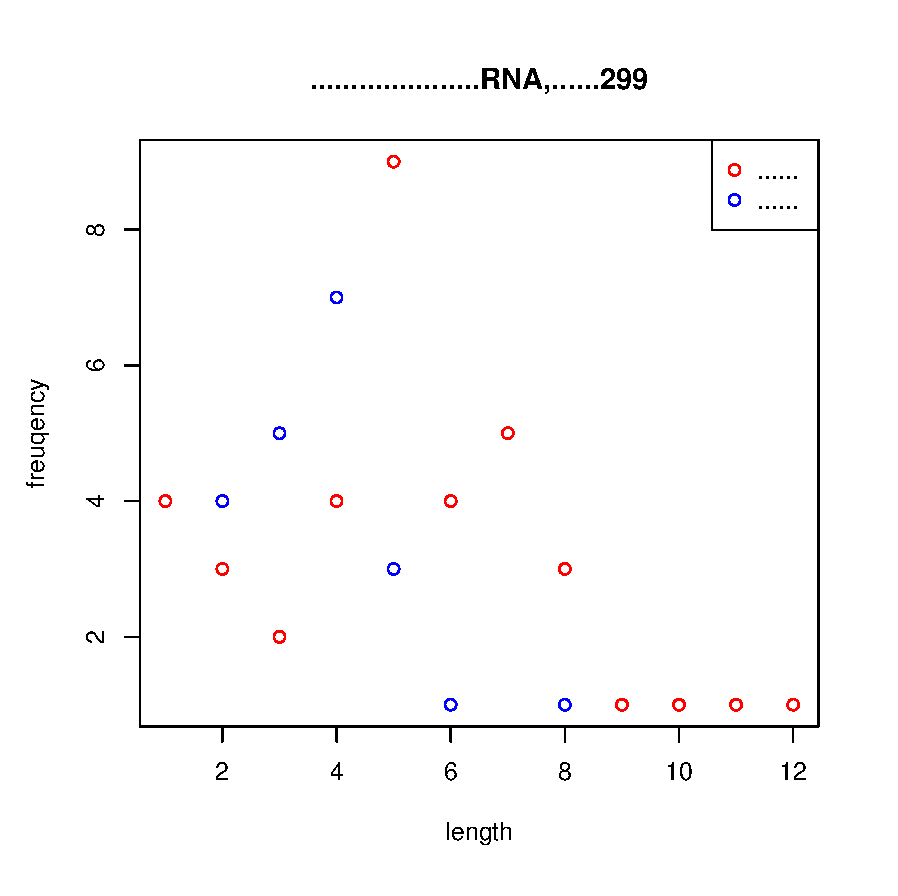
\includegraphics{Plotting2.eps}
\end{figure}
\section{\textbf{\fontsize{12pt}{\baselineskip}{参考文献}}}
\begin{thebibliography}{}
\bibitem{Bib1}    
 生物信息学
 
\end{thebibliography}
\end{document}